\subsection{日本:妖怪与家族象征}
在日本民间传说中,蚰蜒(ゲジ)被视为``家付き神''(家宅精灵)的化身,既能护宅亦能作祟。传说百足蚰蜒修炼千年可化身为``女郎蜘蛛'',象征执念与贪欲。
\begin{figure}[H]
    \centering
    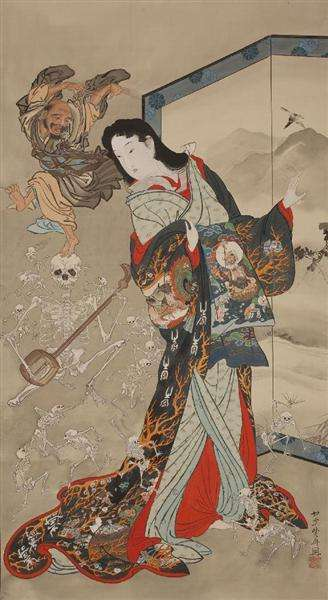
\includegraphics[width = .4\textwidth]{../assets/1.0/图一:河锅晓斋《地狱太夫图》.jpg}
    \caption{河锅晓斋所绘《地狱太夫图》}
\end{figure}

\subsection{欧洲:无害的``屋虫''}
西方文化中,蚰蜒被视为清除蚊虫的益虫,无强烈文化寓意。但因其外形可怖,维多利亚时期小说常以蚰蜒爬过尸体渲染恐怖氛围。